\documentclass[a4paper, twoside, openright]{book}

\usepackage[a4paper, top=2.5cm, bottom=2.5cm, left=2.5cm, right=2.5cm, centering]{geometry}

\usepackage[american]{babel}

\usepackage[bibstyle=authoryear, citestyle=apa, dashed=false, backend=biber, block=space, language=english]{biblatex}
\usepackage{csquotes}

\addbibresource{bibliography.bib}

\renewcommand{\thefigure}{\arabic{figure}}

\renewcommand{\thetable}{\arabic{table}}

\usepackage{graphicx}

\usepackage{subcaption}

\usepackage{hyperref}

\usepackage{titlesec}

\usepackage{fancyhdr}

\usepackage{emptypage}

\usepackage{amsmath}

\usepackage{float}

\usepackage{ragged2e}

\usepackage{pdfpages}

\usepackage[toc]{appendix}

\linespread{1.5}

\setcounter{secnumdepth}{3}
\setcounter{tocdepth}{3}

\titleformat{\chapter}
{\normalfont\huge\bfseries}{\thechapter.}{0.5em}{\huge}

\titlespacing*{\chapter}{0pt}{-40pt}{25pt}

\titleformat{\paragraph}
{\normalfont\normalsize\bfseries}{\theparagraph}{1em}{\normalsize}
\titlespacing*{\paragraph}
{0pt}{3.25ex plus 1ex minus .2ex}{1.5ex plus .2ex}

\pagestyle{fancy}
\fancyhf{}
\lhead{\leftmark}
\fancyfoot[R]{\textbf{\thepage}}
\renewcommand{\headrulewidth}{0.4pt} 
\renewcommand{\footrulewidth}{0.4pt}
\setlength{\headheight}{15pt}

\fancypagestyle{plain}{
  \fancyfoot[R]{\textbf{\thepage}}
  \fancyhead{}
  \renewcommand{\headrulewidth}{0pt}
}

\hypersetup{
    colorlinks,
    linkcolor=black,
    filecolor=black,
    urlcolor=black,
    citecolor=black
}

%--------------------------------
\begin{document}

\begin{titlepage}

\begin{figure}[h]
    \begin{subfigure}[h]{0.2\textwidth}
        
\includegraphics[width=\textwidth]{images/ub_logo.png}
    \end{subfigure}
    \hfill
    \begin{subfigure}[h]{0.2\textwidth}
        
\includegraphics[width=\textwidth]{images/uab_logo.png}
    \end{subfigure}
    \hfill
    \begin{subfigure}[h]{0.12\textwidth}
        
\includegraphics[width=\textwidth]{images/uni_girona.png}
    \end{subfigure}
    \hfill
    \begin{subfigure}[h]{0.2\textwidth}
        
\includegraphics[width=\textwidth]{images/upf_logo.png}
    \end{subfigure}
    \hfill
    \begin{subfigure}[h]{0.2\textwidth}
        
\includegraphics[width=\textwidth]{images/urv_logo.png}
    \end{subfigure}
\end{figure}


\begin{figure}[h]
    \centering
    
\includegraphics[width=0.4\textwidth]{images/logo ccil.png}
\end{figure}

\vspace{4mm}
\begin{center}
  {\LARGE{MASTER IN COGNITIVE SCIENCE AND LANGUAGE}}
  \vspace{7mm}
  \\ {\large\textbf{MASTER THESIS}}
  \vspace{4mm}
  \\ {\Large{September 2024}}
\end{center}

\vspace{15mm}
\begin{center}
  {\Large\textbf{Specific contributions of cortical cortex on the integration of audio-visual walking inputs in patients with stroke compared to healthy subjects: an EEG frequency-tagging approach}}
  \vspace{15mm}
  \\ {\Large{by \textit{Emma Franchino}}}
\end{center}
\vspace{17mm}

\begin{center}
  {\Large{{Under the supervision of:}\\ \textit{Antoni Rodriguez-Fornells \\ Marta Matamala-Gómez}}}
\end{center}

\vspace{4mm}
\begin{figure}[h]
    \centering
    
\includegraphics[width=0.15\textwidth]{images/Picture 1.jpg}
\end{figure}

\end{titlepage}

\cleardoublepage
\newpage 
\thispagestyle{empty}
\begin{flushleft}
  \vspace*{15em}
  \justify
  \textbf{Abstract}: The brain dynamics underlying sensorimotor synchronization constitute a complex combination of different neural processes. Here we wanted to investigate the contribution of cortical cortex on rhythmic sensorimotor synchronization when coupling with auditory and visual inputs related to walking movement. The study has a mixed-models study design with auditory (footsteps sound) and visual (point-light figure) inputs set at the frequency rate of 2 Hz. They were used in three different blocks: audio, audiovisual and visual. The study was conducted by means of electroencephalography (EEG) in a frequency-tagging approach on two distinct groups of individuals: healthy control subjects (\textit{N = 21}) and patients with a stroke (\textit{N = 21}). The results of both population groups showed neural responses of the sensorimotor area in all the stimuli presented in a rhythmic condition, though not in the random one. Such outcome is sustained by behavioral questions on the positive feeling towards the distinct stimuli, which appeared with significantly higher values for the inputs repeated in the rhythmic condition. Moreover, sensorimotor synchronization appeared in auditory and audiovisual inputs, but not in the visual one. In the stroke population the neural response patterns resulted weaker than in the control group, and left-lateralized. These results demonstrate that the sensorimotor synchronization can be elicited only by sensory stimuli repeated in a rhythmic sequence and that auditory inputs appear better to induce neural entrainment. Furthermore, it could be concluded that stroke patients preserved the ability of sensory integration and neural entrainment, even if it results reduced compared to healthy individuals. 
  \vspace*{3em}
  \justify
  \textbf{Keywords}: EEG, Frequency-tagging, Stroke, Sensorimotor integration
\end{flushleft}

\tableofcontents

\chapter*{Acknowledgements}
I am indebted to my advisors Marta Matamala-Gomez and Antoni Rodriguez-Fornells, for the guidance and precious suggestions that they gave me during the whole process of collecting and analyzing the data, as well as the writing of the thesis. \\
I also would like to thank David Cucurell Vega from the Cognition and Brain Plasticity Unit for his precious support and patience during the EEG analysis. \\
The thanksgiving is also extended to the whole laboratory of Bellvitge for the warm welcoming and the important insights, which helped with the research. \\
Then, I want to thank my friends, from the ones of a lifetime to the ones who I just met this year, who make life funnier and never make me feel lonely. \\
I give my most profound thank you to my family, who supported me in every step of my academic carrier and always make me feel loved. \\ A huge gratitude and love goes to my Umbi who has helped me during the process of this thesis in both technical aspects, and especially in the emotional ones. \\
Finally, this work is dedicated to nonno Piero, who I know would be proud.

\chapter{Introduction}
%%% general introduction on stroke
%% stroke incidence
An average of 5.5 million people worldwide die every year because of a stroke, ranking it as the second leading cause of death and one of the main cardiovascular diseases \parencite{Donkor_2018}. Research in the United States has stated that more than 795,000 people have a stroke every year, that is almost one person every forty seconds \parencite{Tsao_2023}. In the past three decades, an increase in the incidence of stroke was globally observed, especially in young (18-44 years old) and mid-life (45-64 years old) populations, yet not in older adults (over 65); on the other hand, the incidence of death and disability has decreased as a result of the advance of research and medicine \parencite{Yahya_2020}. \\
Even though a decrease in disability has been observed, stroke remains the leading cause of serious long-term disability: more than 50\% of people who survived a stroke become chronically disabled, both in neurological and physical aspects. One of the most common consequences is long-term motor impairment due to lesions in cortical or subcortical motor areas \parencite{Karthikeyan_2019}. 

%% stroke: ischemic and hemorrhagic // cortical subcortical
Stroke is divided in two main subtypes, drawn by the cause of it. The most common one results to be the ischemic stroke, it's produced by a blockage of blood vessels and comprehends TIAs (transient ischemic attacks) or mini-strokes, which only last for a few minutes up to 24 hours. The second type is the hemorrhagic stroke which is caused by bleeding in or around the brain, and it appears to cover just the 15\% of the cases \parencite{Abdu_2021}. \\
On the other hand, if we look at the brain regions lesioned by stroke, it's possible to differentiate it between cortical and subcortical injuries, which can alter different cognitive (e.g. language, space orientation) and physical abilities (e.g. motor impairment, weakness), depending on the specific cerebral area and lobe affected. 

%% Gait impairment
One of the major consequences of experiencing a stroke is impaired gait: a total of 80\% of patients have an impaired walking ability, with 50\% of patients who are completely unable to walk, 12\% who can walk with assistance, and 37\% can walk independently \parencite{Balaban_2014}. In those cases, gait can result as hemiplegic, slower in speed and cadence and as well as shorter stride length \parencite{Gomez_2020}. The balance of the locomotor control is shift due to the lesion in the central nervous system (CNS) affecting automaticity, proprioception, balance, anxiety state and multisensory feedback, which will impair walking abilities \parencite{Clark_2015}. 

Due to the wide spreading of gait impairment in patients who suffered from a stroke, the recovery of walking ability is of the main aims in stroke rehabilitation. Recently rehabilitation techniques have been moving towards top-down approaches, which base the rehabilitation on the state of the brain after stroke. These techniques use a motor learning approach mainly through the integration of sensory feedback, helping the proprioception of the body thanks to sensory-motor adaption \parencite{Belda-Lois_2011}. \\
Auditory feedback has been a fundamental sensory feedback for gait rehabilitation, being used as a real-time cue to correct movement and redirect walking. Both auditory and visual stimuli have been employed in different neurophysiological rehabilitation techniques, such as in Proprioceptive neuromuscular facilitation (PNF) \parencite{Moros_2000} or Motor Imagery (MI) \parencite{Mason_2007}. \\
Movement sonification has also been engaged, here the physical properties of the human movement are being translated to audio parameter (e.g. the speed or position of the body are translated into volume or timbre of audio sounds) \parencite{Effenberg_2016}, enhancing motor learning based on motor perception and its representation \parencite{Bevilacqua_2016}.

Sensory feedback employed for movement rehabilitation induce biological motion perception. Studying the neurological processes that underline motion perception, results as a complex goal, since multiple social cues perception and process are involved. In order to isolate only the interested brain activity related to motor perception a new paradigm studying neural entrainment through electroencephalogram with a frequency-tagging approach, with a neutral visual stimulus of a point-light figure walking, has been proposed by \cite{Cracco_2022}. 

%% neural entrainment: definition
Neural entrainment or sensorimotor synchronization is defined as unidirectional synchronization of neural oscillations to an external rhythmic stimulus \parencite{Lakatos_2019, Haegens_2018}; an action is rhythmically coordinated with a predictable external stimulus \parencite{Pressing_1999}. We use rhythmic synchronization between the auditory and motor systems in many of our everyday behaviors, one of the main being speech. Our brain leans towards a natural synchronization of its movement with endogenous rhythmic signals: auditory rhythms rapidly entrain motor responses into stable steady synchronization states \parencite{Thaut_2003}. Such alignment of motor and sensory rhythm at the neural level can be detected in music, dance, sports, rhythmic tasks and verbal communication \parencite{Rosso_2023}. Sensorimotor entrainment can be driven by a status of phase- and frequency-locking of neural oscillations, which will reflect the changes in the external sensory through neuronal excitability \parencite{Lakatos_2005}. 

%% frequency tagging approach (what is it and why it looks like the best methodology)
A way that has been found successful to study neural entrainment is the frequency-tagging approach, where a brain response is elicited through a repeated cycle movement; if the aim is movement perception related to walking the brain response can be elicited at the end of every footstep \parencite{Cracco_2022}. The cognitive and sensory processes present in neural entrainment (brain synchronization with the sensory input presented) are represented by neural oscillations that can be observed through electroencephalography (EEG): EEG signals result in time-locked to re-occurring sensory stimuli \parencite{Thut_2012}. \\
State-of-the-art approaches tag frequencies of a rhythmic stimulation in the power spectrum of EEG in order to quantify neural entrainment \parencite{Nozaradan_2011}: the "frequency tagging" methodology converts brain signals into their frequency components. 

%% rhythmic audio and visual stimuli to activate sensorimotor cortex
The usage of frequency tagging with electroencephalography results in the most appropriate technique to study the role of different brain regions integrating multisensory stimuli through neural entrainment, being able to isolate the brain processes related to movement perception, distinguishing them from other cognitive processes that may be related to social cues using neutral sensory inputs, such as a point-light figure with no gender, weight nor emotional trait \parencite{Cracco_2022}. \\
Brain synchronization remains a complex phenomenon, previous research showed that listening to repeated rhythmic beats activates cortical oscillation evoked from auditory stimuli and anticipations of it \parencite{Snyder_2005}. The different brain regions that are being enhanced during auditory-motor entrainment include: the cerebellum \parencite{Grahn_2011}, inferior colliculus \parencite{Tierney_2013}, basal ganglia \parencite{Thaut_2009} and cortical hubs, located at the top cortical networks, that enable sensorimotor integration.

%% aim of the study
In conclusion, research proved that the auditory and visual feedback can elicit motor responses by neural entrainment in the motor cortex, generating synchronized brain oscillations to the rhythm of the stimuli; furthermore different studies demonstrated that such feedbacks play a key role in stroke gait rehabilitation \parencite{Chen_2018}, facilitating motor automaticity, redirection and action.

Even if gait rehabilitation in stroke results much investigated, not many studies have examined the neural activation related to the integration of multisensory feedback. For this reason the aim of the present study is to research the brain dynamics supporting the sensorimotor synchronization when coupling auditory and visual inputs related to walking movement, comparing control healthy subjects and patients who suffered from a stroke. \\
The study will be conducted using electroencephalogram frequency tagging approach, aiming to elicit neural entrainment with visual and auditory stimuli related to gait at the frequency of 2 Hz, which has been proven to be the most indicated to activate the sensorimotor cortex in healthy subjects, especially with the use of rhythmic auditory stimuli, by previous study (Matamala-Goméz et al. in preparation).\\
Looking at the results of the previous study conducted with multiple frequencies only on healthy subjects, we expect to find a higher brain activation related to the auditory inputs played at 2 Hz, with an activation of the temporal and sensorimotor cortex. On the other hand, for the visual stimuli we expect an activation of the occipital area and a weaker elicitation of the sensorimotor cortex. For all the sensory inputs we predict to see a significant higher neural synchronization in the stimuli a rhythmic sequence rather than in a random one. \\
Finally, for what concerns the results related to the stroke population, we may see some difference from the control group in the brain activation due to the brain injuries that they've suffered: a lateralized arousal in the contralateral area of the lesion, or a contrast in the intensity of such arousal could be observed.

% Yet, since cortical and subcortical areas were depicted as facilitators for motor alignment thanks to the ability of beat-based time-keeping \parencite{Cannon_2021}, we expect differences of brain activation in stroke patients compared to healthy subjects, but still, visible neural entrainment elicited by repeated rhythmic multisensory stimuli. 

\chapter{Methods}
\section{Participants}
In the present study, we had a total population of 42 subjects, equally divided into two groups: 21 individuals were part of the healthy control group, whilst the remaining 21 were patients who suffered from a cortical or subcortical stroke. The recruitment for the control group was made through several methods: in person, talking to alumni of the \href{https://www.experiencia.ub.edu/ca/}{Universitat de l'Experiència of Barcelona}, through personal contacts, and using the platform \href{https://www.sona-systems.com/}{Sonasystem}. 
On the other hand, to recruit participants who experienced a stroke we used a database previously employed in another study made in the \href{https://brainvitge.org/}{Cognition and Brain Plasticity Unit} for movement rehabilitation with music therapy. Furthermore, we were also able to present our study at \href{https://www.fundacioictus.com/}{Fundació Ictus}, where we could select more participants.  
The exclusion criteria in both groups were: no visual or auditory impairments and no pregnancy.

Participants of the two groups were matched by age and gender, where we can find a mean of 55,4 years old in the control group and of 56,4 for the stroke patients, with a non-significant difference (\textit{t} test: -0.299, \textit{p} value: .766). Likewise, the difference is gender did not result significantly different (\textit{t} test: 1.56, \textit{p} value: .127), even though higher participation of men compared to women can be observed in the stroke group and a preponderance of women compared to men can be observed in the control group. 
To both groups a questionnaire measuring the level of physical activity was administrated: an average of 7026,78 kilojoules a day was found for the control group, whilst for the stroke group it resulted of 5669,19 kJ/d, which results lower than the control group, but still without a significant difference (\textit{t} test: 1.06, \textit{p} value: .146). 
Regarding the stroke group, the clinical history of the patients was collected, founding the majority of patients with the injured left hemisphere, which affected their contralateral right extremity (\textit{N=}13 suffered the injury in the left hemisphere; \textit{N=}7 in the right hemisphere; \textit{N=}1 in both hemispheres; a database can be found in Table A.\ref{tab: Database stroke}). 
Participants signed an informed consent before the experiment, and they were reimbursed for their time. 
% This study was conducted according to the ethical rules presented in the General Ethical Protocol of the Faculty of Psychology and Educational Sciences.

\section{Materials}
The experiment was conducted with electroencephalography, recorded using a standard set-up with 64 Ag-AgCl electrodes placed on the scalp according to the International 10/10 system (\href{https://www.easycap.de/}{EasyCap}) to capture the neural activity in the whole brain. 
The study presented auditory (footsteps sounds) and visual (point-light-figure) inputs (Figure \ref{fig: visual stimuli}) related to the walking ability, all set at the frequency of 2 Hz, using Matlab for the visual stimuli and \href{https://www.audacityteam.org/}{Audacity software} for the auditory ones; resulting the best to activate neural entrainment (Matamala-Gomez et al. in preparation).

For what concerns the visual stimuli, a point-light figure walking, representing the human body through white dots set in the primary joints of the body (Figure: \ref{fig: visual stimuli}), was used: it was created with \href{https://www.biomotionlab.ca/html5-bml-walker/}{BioMotionLab}, using a neutral subject, without any specific gender nor emotional display, with an average weight. After being created with the mentioned software, its frequency was adjusted to the desired one. The choice of a neutral point-light figure as the visual stimulus was made to focus only on brain activity elicited by movement processing frequency. Earlier studies have in fact shown that the presence of different important biological and social features can be inferred from figures and may enhance other processes not primarily related to movement perception \parencite{Cracco_2022}. 
For the audio stimuli, the sound of footsteps at 2 Hz with a neutral connotation was engaged. The participants listened to the sound through headphones and they were asked to pay attention to the blue fixation cross displayed in the middle of the black screen. 
Finally, a third stimulus consisting of the union of the point-light figure walking and the sounds of the footsteps, was employed and denominated as audiovisual. 
\begin{figure}[h]
    \centering
        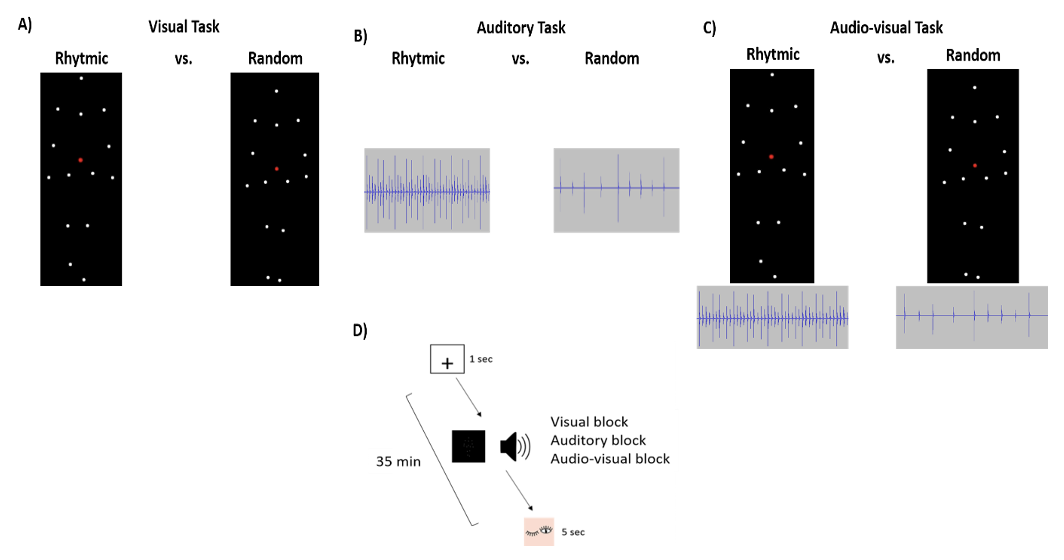
\includegraphics[width=0.85\textwidth]{appendix/Picture 1.png}
        \caption{Auditory, visual, audiovisual inputs, and the experimental timeline}
        \label{fig: visual stimuli}
\end{figure} 
Moreover, after the observation of each sensory input, six subjective report questions were presented: they referred to how the participant felt while seeing the point-light figure walking or listening to the footsteps sound. The questions had to be answered on a Likert scale with values between 1 (strongly disagree) to 5 (strongly agree) (see the Experimental Design section for further details and (Table \ref{tab: Behavioral questions})). 
The experimental task was developed using with \href{https://pstnet.com/products/e-prime/}{E-prime} software, which allowed us to build an experiment with different stimuli presentations (e.g. adding images, questions and text).

To measure the level of physical activity of each participant, which would be later correlated to the EEG results, we used the \textit{Active-Q} questionnaire (it can be found in the Appendix A.(\ref{pdf: Active-Q questionnaire})), which was created precisely to assess the total physical activity and inactivity in adults, through a series of multiple choice questions (referred to a one-year time) on daily activity, mean of transportation used, leisure and sports activities; and the time a day spent for each of them \parencite{Bonn_2012}. 
The questionnaire was translated in Spanish from the original English version and transformed from a PDF file into an interactive digital version using the platform \href{https://www.qualtrics.com/uk/?rid=ip&prevsite=en&newsite=uk&geo=ES&geomatch=uk}{Qualtrics}. 

\section{Experimental design}
The current study is a mix models study design presenting both auditory (footstep sound) and visual (walking point-light figure) inputs at the frequency rate of 2 Hz in a rhythmic or random sequence, in three different blocks (auditory, visual and audiovisual). The blocks were presented in a randomized order to all the participants. 
At the beginning of the experimental session, we included a text with the instructions and right afterwards a white fixation cross preceding each sensory input presentation. 
In each experimental block the sensory inputs were presented four times in rhythmic sequences and four times in random sequences, each sensory input presentation lasted 60 seconds. The sensory inputs were presented in rhythmic and random sequences in a random order within each experimental block.  

During the presentation of each sensory input an attentional task was set. For the auditory inputs, the participants had to detect changes of the pitch (to a more acute or grave footstep sound) in the footstep sound stimuli. For the visual and audiovisual inputs, the participants had to focus their attention on the central dot of the point-light-figure which changed from red to white. The participants had to report to the experimenter the number of changes in both pitch footstep sound and the color of the central dot after each sensory input presentation.  
Moreover, after each sensory input presentation the participants had to answer six subjective report questions in a 5-points Likert scale (see Table \ref{tab: Behavioral questions}). Finally, after answering the subjective report questions, an eye-blink figure was presented during fifteen seconds indicating that they had time to blink if needed (see Figure \ref{fig: visual stimuli} for the experimental block design).  
A break of roughly five minutes was taken between all blocks to fix the conductivity of the electrodes with a gel \footnote{The gel employed in the EEG procedure is a mix of salts and water that allows the conductivity between the scalp and the electrodes.} and to let the participants rest. Altogether, the experiment and the set-up of the EEG cap on the participants had a duration of almost two hours.

For what concerns the Active-Q questionnaire, it was administrated via e-mail a few days before the experiment, together with some additional information about the study.

\section{Procedure}
Before the experiment began the participants had to sign the informative consent, and they would ask questions if needed. Afterwards a careful preparation was made, where we placed the EEG cap on their head\footnote{The EEG cap was previously prepared with all the 64 electrodes in their relative site.}, the external on the side of the right eye and under it, as well as on the mastoids. Then a gel was inserted in each electrode (both external and placed on the cap) in order to diminish the impedance and allow a good signal connectivity. 
Additionally, if the participants had any trouble completing the Active-Q questionnaire at home, they were helped to do so before the start of the experimental session. 

The participants sat on a chair in front of the computer screen where the stimuli were displayed and wore headphones to listen to the auditory stimuli. They were asked to avoid moving and blinking when the sensory stimuli were presented to avoid noise signal in the EEG recording. 
After reading the instruction on the screen, the participants had to pay attention to the stimulus that was being presented and count the number of changes in the color of the point-light figure's central dot or in the tone of the footstep sounds. At the end of each stimulus, they were asked to tell the experimenter how many changes they were able to observe or hear through a speaker\footnote{The speaker was used to communicate with the participants, which were in a different room from the experimenters. Furthermore, they could be seen through a webcam, and make signs if anything was needed.}. 

Afterwards, the subject questions were presented and had to be answered by the participants using numbers from 1 to 5 on the keyboard placed in front of them. When a question was answered the following one was automatically shown. When all the six questions were completed the eye-blinking image was presented, this was inserted for the participants to yawn, blink or stretch their face muscles if needed; furthermore they were expressively told that they could do so also during the answering of the questions, since the EEG recording during those time was of no interest for our analysis.  

After all the eight stimuli with their relative questions were shown, a block was completed and a small break took place, where the participants were offered something to drink or eat and the electrodes' impedance was checked. 
When all the blocks were completed, the participants could wash their head from the gel in a sink.

\subsection*{Subjective report assessment scale}
For the subjective report questions presented at the end of each experimental block we used six question related to the participant's perception of the sensory inputs, which can be found in Figure \ref{tab: Behavioral questions}. 
We inserted these questions to understand the feelings produced by the sensory inputs; in particular we aimed to see if the perception of involvement with the sensory input or the positive feelings recognized during the presentation of such stimuli, could influence the level of neural entrainment related to that particular sensory input. Further, we wanted to understand if the difference of sensorimotor synchronization previously observed between the presentation of the stimuli presented in a rhythmic or random sequence (Matamala-Gomez et al. in preparation) could also be confirmed by a subjective report on their perception. 
For these purposes, we decided to insert two questions on the involvement of our body with the sensory stimuli presented (Q1 \textit{«I felt involved with the marching movement of the white dot figure during the video observation (it was as if I was also moving)»} and Q4, measuring agency \textit{«During the observation of the video, I felt like I was inside the body of the white dots (as if my own body was performing the movement)»}); two questions on the positive feelings evoked by the stimuli (Q5 \textit{«During the observation of the video, I had a pleasant sensation”} and Q6 \textit{«During the observation of the video, I felt relaxed»}); one on the fluidity of the stimuli (Q3 \textit{«The movement of the white dot figure seemed fluid to me.»}); and one on the perception of the rhythm, which was considered the most significative one (Q2 \textit{«The rhythm of the steps of the white dot figure seemed to reproduce the rhythm of my real march»}). 
All the questions were adapted for each different sensory input, and can be found in Figure \ref{tab: Behavioral questions}. 
Their score had to be given on Likert Scale from 1 (strongly disagree) to 5 (strongly agree). The results obtained from the questions were collected into a \textit{.txt} file by E-prime and inserted in an Excel table through a Python script, so that later they could be easily used to make statistical analysis. 
\begin{table}[H]
    \centering
    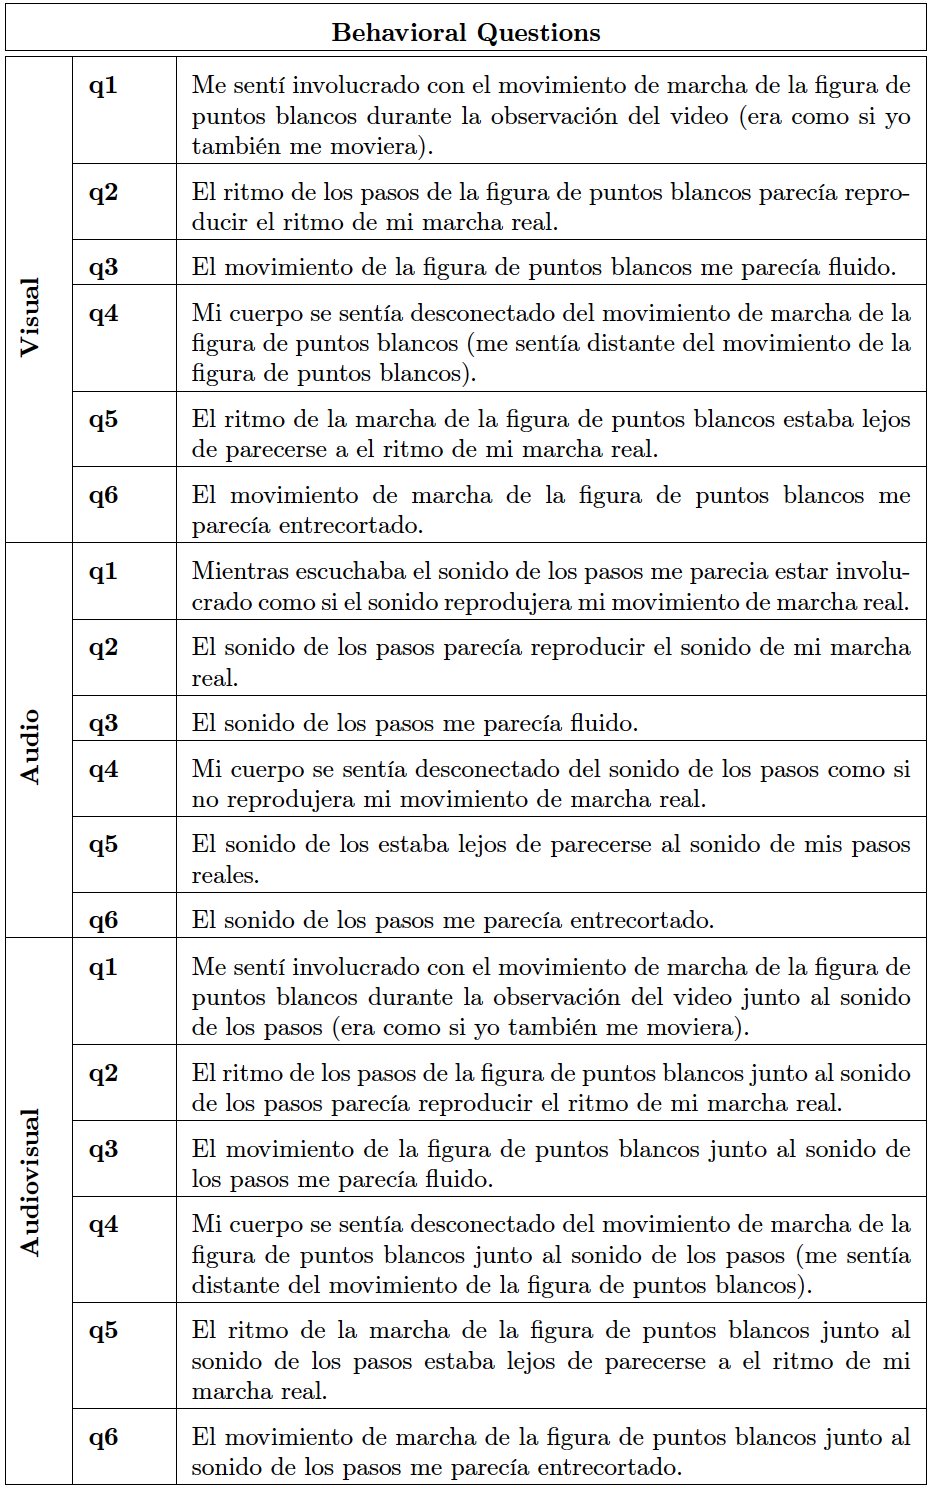
\includegraphics[width=0.65\textwidth]{appendix/questions.png}
    \caption{Table: Subjective report questions translated in English from Spanish}
    \label{tab: Behavioral questions}
\end{table}

Regarding the data for the Active-Q questionnaire (the questionnaire can be found in the Appendix \ref{pdf: Active-Q questionnaire}), we conducted the score calculation following the instruction reported on the article where it is explained, and its efficiency is tested \parencite{Bonn_2012}. Initially, we exported in an Excel file the results collected by Qualtrics with their numeric values (e.g. if the participant had selected the first option, the result would have been 1), this was imported in a Python file where the numeric values related to each activity were transformed into the MET values reported in Table A.\ref{tab: met_values}, which were encountered in the previously cited article. On the other hand, the frequency of each activity was measured multiplying the hours/minutes a day for the number of days per week; if a range of time was presented, we previously calculated the average of it, and then convert it into hours per day (e.g. the range 15-29 minutes/day was converted to 0.36 h/d).  
After creating an Excel table with the new scores accorded to MET values and the duration of hours/week, we proceeded to calculate the final Active-Q score, which returns a number of kilojoules per day, using the following formula: 
\[
\text{EE}_{\text{activity}} \, (\text{kJ/day}) = \text{MET}_{\text{activity}} \cdot \text{Weight} \, (\text{kg}) \cdot \text{Duration}_{\text{activity}} \, (\text{h/d}) \cdot 4.184
\]
The MET value and duration of the activity were multiplied by the weight of each participant (which was asked individually to the participant before the experiment), and the number 4.184, which is a conversion factor used to transform values from kcal to kJ. The obtained results represented the daily physical activity of each participant.

\section{Analysis}
\subsection{EEG data analysis}
The EEG data was registered through the software provided by \href{https://brainvision.com/applications/brain-vision-software/}{BrainVision} at the sampling rate of 1000 Hz; for all the subjects we made three different registrations, one per each experimental block (auditory, visual, and audiovisual). 
Before conducting the frequency-tagging analysis, the data was preprocessed using the \href{https://eeglab.org/}{EEGLAB toolbox} ran with Matlab: all the chunks of register that weren't necessary (i.e. the initial part with the instructions, the one related to the eye-blink figure and the ones corresponding to the subjective report questions) were trimmed. Later we re-referenced the data to channels 31 and 32, which correspond to the electrodes TP9 and TP10, positioned externally on the mastoids. Finally, we ran the Independent Component Analysis (ICA) to remove blinking and muscles artifacts and saved the preprocessed data into a new file. 

After the data for every block and for all the participants was preprocessed, we started the analysis with the help of some scripts made for the previous study and adjusted according to our necessities. 
Firstly, we extracted the epochs from the processed data: epochs of 20 seconds were obtained from the 60 seconds of each stimulus; the method of surface Laplacian and Current-Source Density (CSD) transform was applied to the data, dividing it between the one related to the rhythmic stimuli and to the random ones. 
From the files just generated, we computed spectral power activity with \href{https://www.fieldtriptoolbox.org/}{FieldTrip toolbox} of Matlab, using \textit{mtmfft} method, which allowed performing later analysis in time and frequency domains to study oscillatory brain activity and its modulation over time. The Fast Fourier transform (FFT) was applied to each sensory input (visual, audio and audiovisual) in both rhythmic and random sequences; therefore six variables were obtained. 

Using these variables we computed the averaged Signal-to-Noise Ratio (SNR), calculating the averaged signal-to-noise ratio (SNR) and the mean power spectrum and its variance through the different frequencies. We also plotted the activity power spectrum to see how the neural synchronization to rhythm would change through frequencies, and to observe whether the desired peak amplitude activity at 2 Hz was present. 
For the activity power spectrum analysis we decided to take into considerations the different regions of interest (ROIs) of our experiment, concerning the Occipital, Temporal and Sensorimotor areas, respectively enhanced by visual and audio sensory inputs as well as motor synchronization. For the analyses, the three different ROIs included the following electrodes: Temporal (right: FT9, FT7, T7, TP7; left: FT10, FT8, T8, TP8), Sensorimotor (right: F5, F3, F1, FC5, FC3, FC1, C5, C3, C1; left: F2, F4, F6, FC2, FC4, FC6, C2, C4, C6), and Occipital (PO3, POz, PO4, O1, Oz, O2). 

Furthermore, in order to neutralize the effects that the side of the injury in stroke patients might have on our results, we decided to invert the location of the electrodes for the patients who suffered the lesion in right hemisphere, which were the minority. Doing so the topographies that were generated should result not affected by the different injured side of the brain and the left hemisphere becomes the Affected Hemisphere in the stroke group and the Right hemisphere would be the Unaffected hemisphere. The interpretation of the corresponding figures in the results' section should be in consideration this aspect.  

Finally, we observed the distribution of the power spectrum activity for each sensory input, in both rhythmic and random sequences for each experimental block when presenting the sensory input at 2 Hz, in healthy individuals and patients with stroke. Moreover, we also could observe the power spectrum activity difference between rhythmic and random sequences (Figures \ref{fig: 3D topographies control group} and \ref{fig: 3D topographies stroke group}). 

\subsection{Subjective report questions analysis}
For the subjective report questions, we analyzed the mean difference between rhythmic and random sequences in each experimental block (auditory, visual, and audiovisual) for each subjective report question of the questionnaire. Further, we also calculated the mean difference between healthy subjects and patients with stroke in both rhythmic and random sequences in each experimental block for each subjective report question (Figure \ref{fig: bar_visual_pop}). In specific, we used the Wilcoxon Signed-Rank test for non-normally distributed data or the paired T-test for normal distributed data. We tested the distribution of the data with the Shapiro–Wilk test.
% We inserted all of our statistic results for each group and sensory input into different Excel tables in order to build with them separate bar plots (with their corresponding error bars) to show graphically the comparison between the rhythmic and random condition. 
% Finally, we decided to achieve an additional comparison between the rhythmic and random condition in the two distinct population groups, building a single bar plot with the mean results of all the questions in the diverse stimuli in the two groups. 

%% ---- questionnaire analysis part 
On the other side, with the scores of the physical activity, obtained with the Active-Q questionnaire, we aimed to explore the relationship with the subjective report questions and the brain power spectrum. To that aim we used Spearman’s correlation test for non-parametrical data. 
For the correlations, a numerical value for each participant and condition representing the mean power spectrum activity of each specific ROI (temporal, sensorimotor, and occipital) during each sensory input exposure (auditory, visual, and audiovisual) only at rhythmic sequences, was extracted, in both healthy and patients with stroke. 
In order to see whether there was a relationship between the power spectrum activity and behavioral responses, we selected the question Q2 (see Table \ref{tab: Behavioral questions}), that was the one more related to the rhythmic perception of the sensory input presentation. 

\chapter{Results}
\section{EEG results}
The outcome of our EEG analysis are descriptive EEG results, which will be deepened later, through advanced statistical analysis.\\ 
At beginning of our EEG data analysis we plotted the averaged signal-to-noise ratio (SNR) to observe if the desired brain signal would have been distinguishable from the background EEG activity. We can observe our plots of the rhythmic and random conditions of the two population groups in Figure \ref{fig: snr_rhythmic: control} and \ref{fig: snr_rhythmic: stroke} for the rhythmic condition and in Figure \ref{fig: snr_random: control} and \ref{fig: snr_random: stroke} for the random one. \\
The graphs don't seem to differ much between control and stroke groups.  The rhythmic conditions, in which the frequency has been precisely set at 2 Hz, show the highest peak at 2 Hz and its harmonic (4 Hz), while a flat SNR values for what concerns the other frequency. An exception regards the frequency of 1 Hz were the SNR appears still lower than the interested peaks, but higher than the other non target frequencies. On the other hand, in the SNR related to the random conditions it is possible to detect higher peaks at frequency of 1 Hz and its harmonics 2, 3 and 4 together with some lower noise in all the other frequencies. 

We proceeded to calculate how the power spectrum representing the brain activity of our participant would change across our three regions of interest (occipital, temporal and sensorimotor) during the presentation of the different stimuli in the two conditions, expecting from the last results to find a peak amplitude at 2 Hz in the rhythmic condition. We calculated separately for the two different population groups the grand average of the neural activity in the ROIs related to the different stimuli and the two separate conditions. \\
Giving a general look to the plots of all the ROIs (that can be found starting from Figure \ref{fig: occipital ROI: control}) we can see a clear activation peak at 2 Hz in the rhythmic conditions and not in random ones for both of the population groups, as expected. However, it is also noticeable that the peaks found in all the ROIs power spectrum of the stroke group appear as lower than in the control group, denoting a weaker brain activation.  
% For what concerns the stimuli in the random conditions the results appear to be almost the same in all the ROIs including this first one with all the electrodes: the higher power activity can be observed at 1Hz and its harmonics even if with a lower value than the peaks at 2 Hz in the rhythmic conditions.

Observing the plots for the specific ROIs, we can spot in the occipital ROI (Figures \ref{fig: occipital ROI: control} and \ref{fig: 3D topographies stroke group}) it is possible to spot the peak at 2 Hz clearly in the rhythmic condition of the visual and audiovisual sensory inputs, whilst in the temporal ROI (Figures \ref{fig: temporal ROI: control} and \ref{fig: temporal ROI: stroke}) it can mainly be observed it in the audio and audiovisual rhythmic conditions. Considering the last ROI, the sensorimotor area (Figures \ref{fig: sensorimotor ROI: control} and \ref{fig: sensorimotor ROI: stroke}), the activity peak at 2 Hz can only be noticed in the audio and audiovisual rhythmic conditions; in the visual one, a higher brain activity is spotted only in the control group at 1 Hz, similarly to its activity power spectrum in the temporal ROI.

Having the desired graphs representing the activity power spectrum over frequencies, we proceeded to plot the two- and three-dimensional topographies concerning the brain activity of the different population groups, just in the specific frequency of 2 Hz, related to the three different stimuli, for both the rhythmic and random conditions, adding the difference between these two. \\
In Figure \ref{fig: topographies control group} and Figure \ref{fig: 3D topographies control group} we can analyze the neural activity of the control group: a strong activation of the temporal and sensorimotor areas were observed both in the audio and audiovisual rhythmic conditions, with a broader spread of the activity in the surrounding areas in the audio condition and the supplementary activation of the occipital lobe in the during the audiovisual stimuli. For what concerns the brain activation during the rhythmic visual stimuli, it can be seen clearly only in the occipital area. \\
Moving to the topographies related to the random condition, the pattern of the brain activation appears as much weaker than the rhythmic condition, with a feeble arousal in some different brain regions. \\
We can conclude that the frequency tagging effect is greater in the rhythmic conditions, with an activation of the ROIs that can be detected through the difference between the two conditions. 

For what concerns the stroke population the encountered results (Figure \ref{fig: topographies stroke group} and Figure \ref{fig: 3D topographies stroke group}) appear as slightly different from the control group. During the audio stimuli, the temporal and sensorimotor areas looked activated, even if not as much as in the control group. Furthermore, strong lateralized arousal on the left side of the brain can be denoted in both the topographies related to the audio and audiovisual stimuli. On the other hand, the visual stimuli elicited a weaker activity in the stroke population compared to the control group, as well as a softer left sided activation than the audio and audiovisual ones. \\
As in the control group, the random condition present a general weak brain activation, with the main difference of a noticeable arousal for what concerns the left side lateralization. \\
Finally, the difference between the two conditions confirms the activation of the diverse ROIs related to the corresponding sensory inputs, resulting more feeble than the ones found in the control group. 

\section{Behavioral results}
For the analysis of the behavioral results, we firstly made various bar plots divided for population groups and sensory inputs. Firstly, in Figures \ref{fig: bar_visual_control}, \ref{fig: bar_audio_control} and \ref{fig: bar_audiovisual_control}, we can find the results related to the control group: here we can see that all the questions related to every sensory stimulus differ significantly between the random and rhythmic conditions, with higher values for the rhythmic condition. These results are confirmed by the report \textit{p} value in the statistical table in Figure \ref{fig: significance_control_pop}. \\
From the graphical representation and the statistical results we can also detect that the question with the higher values in the rhythmic condition results to be the third one in all the stimuli, which refers to the perception of the movement fluidity by the subject. While this question appears as the one expressing the biggest difference between the two conditions, the last three question in every sensory inputs (q4, q5 and q6) emerge to be the ones with lower differences between random and rhythmic, still being significant.

Moving on to the outcome of the questions answered by the stroke group, which can be found in Figures: \ref{fig: bar_visual_stroke}, \ref{fig: bar_audio_stroke} and \ref{fig: bar_audiovisual_stroke}, similar results to the control group can be observed, with some slight differences. Firstly, we can affirm that equally to the previous results, a significant difference between all the questions related to the random and rhythmic for each sensory input, can be found (Figure \ref{fig: significance_stroke_pop}). \\ However, in the stroke population we can see that the difference appears to be generally lower compared to the one observed in the control group, except for question three in all the sensory inputs, question four in the audio stimulus and five in the audiovisual one. In general, we can conclude that the Likert values assigned to the questions referred to the random stimuli of all the sensory inputs appear as higher than in the control group.

To confirm such difference between the two population groups, we decide to create a plot to visually compare them and to statistically compare their results. In Figure \ref{fig: mean_population_condition} we can recognize the distinction between the answers given by the stroke population and the control one to the random stimuli, and almost identical results for what concerns the rhythmic stimuli. If we then look at the statistical results (Figure \ref{fig: significance_total_mean_pop}) we can detect that the only significant result for the difference between the two population groups can be found for the answers related to the random visual inputs. 

Later, we decided to correlate the most significant rhythmic \footnote{The choice of taking into account only the question in the rhythmic condition was made after seeing the results related to the difference between the two conditions: seeing that the rhythmic one got always higher values than the random.} question (q2) to the mean power activity of the Occipital, Temporal and Sensorimotor ROIs, dividing them always by population group. To represent such correlations we made different scatter plots for each ROI, that can be found from Figure \ref{fig: correlation q2 occipitalROI: control group} for the control group and from Figure \ref{fig: correlation q2 occipitalROI: stroke group} for the stroke group. Additionally, a table with the Spearman coefficient \textit{r} and \textit{p} values can be encountered in Figures \ref{fig: correlation values q2: control} and \ref{fig: correlation values q2: stroke}. 

Looking at the results for the control group we can observe that the scatter plots result quite similar among ROIs, and that no correlation was found between the question related to the various sensory inputs and the power brain activity. The data distribution in all the different plots looks spread, with a bigger concentration towards the higher Likert points and the lower and medium values in the brain activity power spectrum. The lack of correlation between the two variables is demonstrated statistically by the Spearman's coefficient and its \textit{p} values. \\
Contrarily, looking at the results for the stroke population we can find a significant positive correlation between the values assigned to the behavioral question related to the audio stimuli and the neural activation in the Temporal ROI. \\
Moving to the question related to the other sensory inputs (visual and audiovisual), no significant correlation with the mean power activity of the different ROIs could be found just as in the control group.

Finally, we also aimed to understand if a possible correlation between the level of physical activity of the participants and their correspondent mean power activation in the Sensorimotor area could be present. \\
The scatter plots of such correlation can be found in Figures \ref{fig: correlation activeq control} and \ref{fig: correlation activeq stroke}, with their correspondent Spearman values in Table \ref{fig: significance correlation activeq}. \\
The obtained results show no correlation between the two level of physical activity and the activation of the sensorimotor area related to any of the sensory inputs.

\chapter{Discussion}
Discuss your results and their importance, for example, if you have worked with one language would they be applicable to the faculty of language in general? What do your results mean for the theory of language in general? Can they be used to improve speech therapy intervention? Which limitations did you find in your work? Sample size? Uncontrolled variables?

% The observation that target frequencies dominate the spectrum has been commonly taken as evidence for the underlying entrainment of neural oscillations (e.g., Nozaradan et al., 2011 ; Nozaradan et al., 2012 ; Lenc et al., 2018 ), which is not exempt from critiques

% These areas were chosen as ROIs because they were expected to be activated by the various stimuli: the visual stimuli should've activated the occipital ROI, the audio stimuli the temporal ROIs, the audiovisual both of these last ones; meanwhile the sensorimotor area was expected to activate when the neural entrainment would take place. 

\chapter{Conclusion}
The present study provides insights on brain dynamics underlying neural entrainment and sensorimotor synchronization through the frequency-tagging approach with electroencephalogram, in different groups of individuals. The neural tracking in both populations showed higher sensorimotor synchronization in auditory and audiovisual stimuli rather than in the visual one. Further, sensorimotor synchronization, as well as temporal and occipital activation, were delineated with sensory stimuli repeated in a rhythmic sequence rather than a random one, emphasizing the sensorimotor synchronization to periodic beat frequency. Such findings were also supported by the results of the behavioral questions which highlighted the positive feelings of fluidity and involvement with the movement in the rhythmic sequence, whereas these feelings were absent in the random condition. The results for the stroke population were characterized by a diminished and lateralized neural activation compared to the healthy group. \\
Above all, the results of the present study constitute important progress in the knowledge on the role of the cortical cortex on the integration of auditory and visual walking inputs in patients with stroke. The results gave insights on the possibility of employing the same sensory inputs used in the experiment as tool for gait rehabilitation, where sensory feedback have already been proven to be beneficial to enhance motor response \parencite{Bolognini_2016}. Finding strategies to reacquire walking ability and independence from others is crucial for patients. \\
In order to get most appropriate results, that can later be used to adapt sensory inputs specifically for diverse lesion's location, further analysis, taking into account this crucial variable is necessary.

% Other studies have taken into consideration the investigation of sensory integration and motor activation in healthy control subjects (e.g. \parencite{Nozaradan_2011}, \parencite{Nozaradan_2014}), but not many have researched this phenomenon at the neural level in clinical population. 
% Besides, studies in post-stroke walking rehabilitation have demonstrated that sensory (visual, audio and audiovisual) feedback result beneficial to reacquire walking ability. Multisensory integration, which appears to be mostly integrated even in stroke patients, improves enhance motor responses: it helps redirect walking, and rhythmically coordinating action with predictable external stimulus . As for healthy subjects, auditory stimuli have been found to be crucial to activate neural entrainment, especially using movement sonification, i.e. the mapping of movement signals into sound.

% In conclusion, this study provides evidence for the role of attention to auditory input delivered in rhythmic walking sequences in synchronizing auditory areas with the sensorimotor cortex. Specifically, footsteps sound presented at 2 Hz induced a peak amplitude for synchronization with the sensorimotor cortex. Further, when footstep sounds were combined with a walking point-light figure (presented at the same frequency rate), they likely enhanced attention and induced higher synchronization with the sensorimotor cortex. The results from this study may be relevant for designing sensory learning and multisensory integration trainings for motor rehabilitation, based on the neurobiology of rhythmic motor entrainment (Molinari et al. 2003), particularly for the rehabilitation of rhythmic movements such as walking. 

\begin{appendices}
  \fancyhead[L]{APPENDICES}
\appendix

\section{Appendix: Experimental Material}
\begin{figure}[ht]
    \centering
    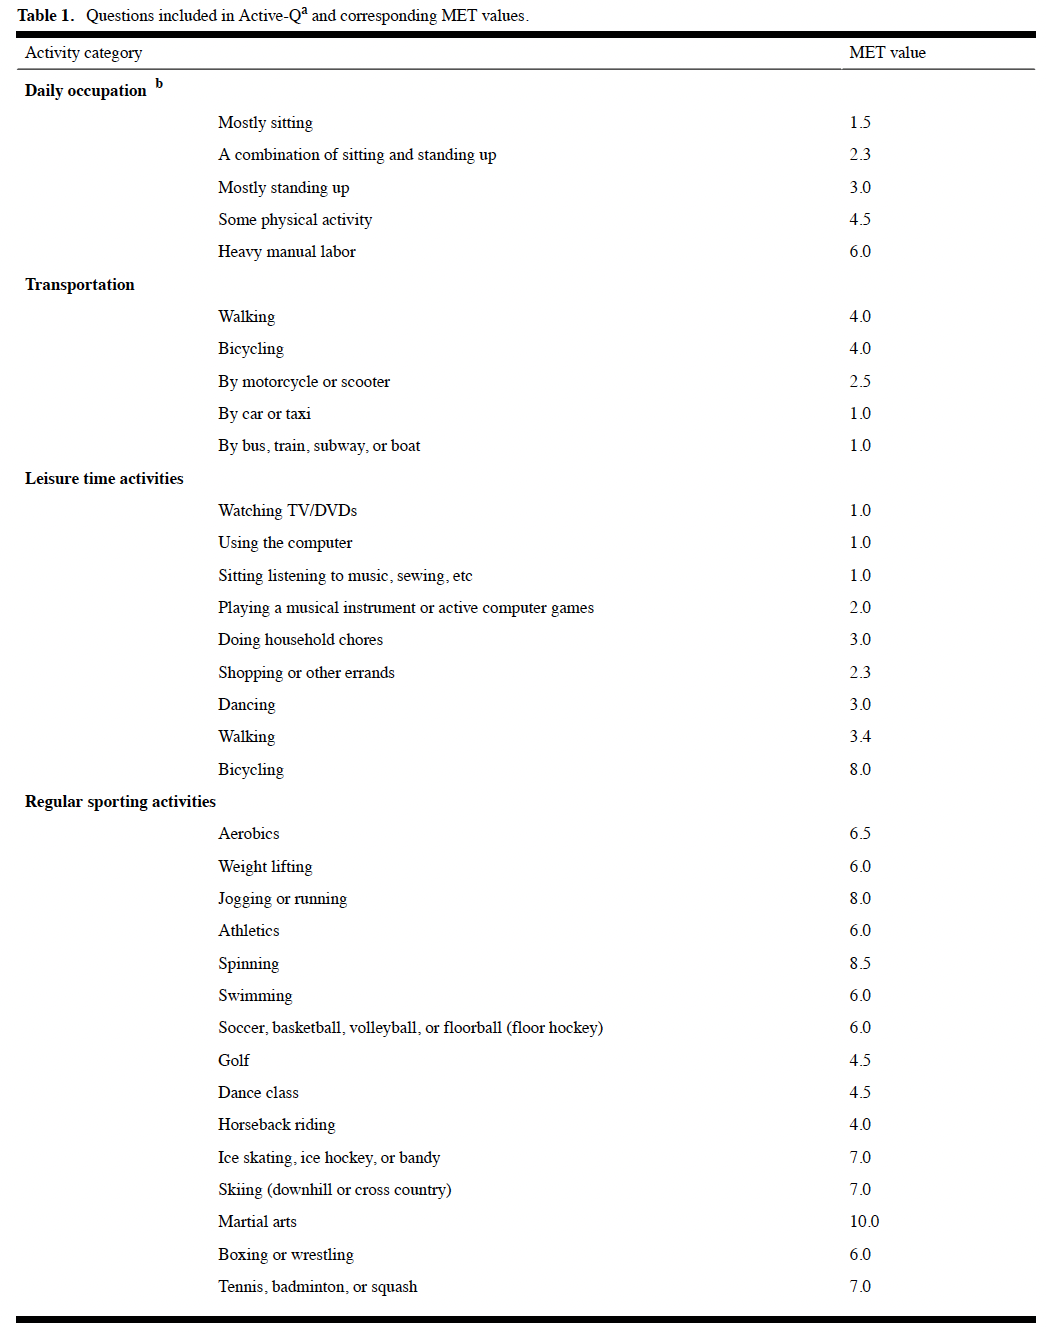
\includegraphics[width=0.8\textwidth]{appendix/met_values.png}
    \caption{MET value labels \parencite{Bonn_2012}}
    \label{fig: met_values}
\end{figure}
\begin{figure}[ht]
    \centering
    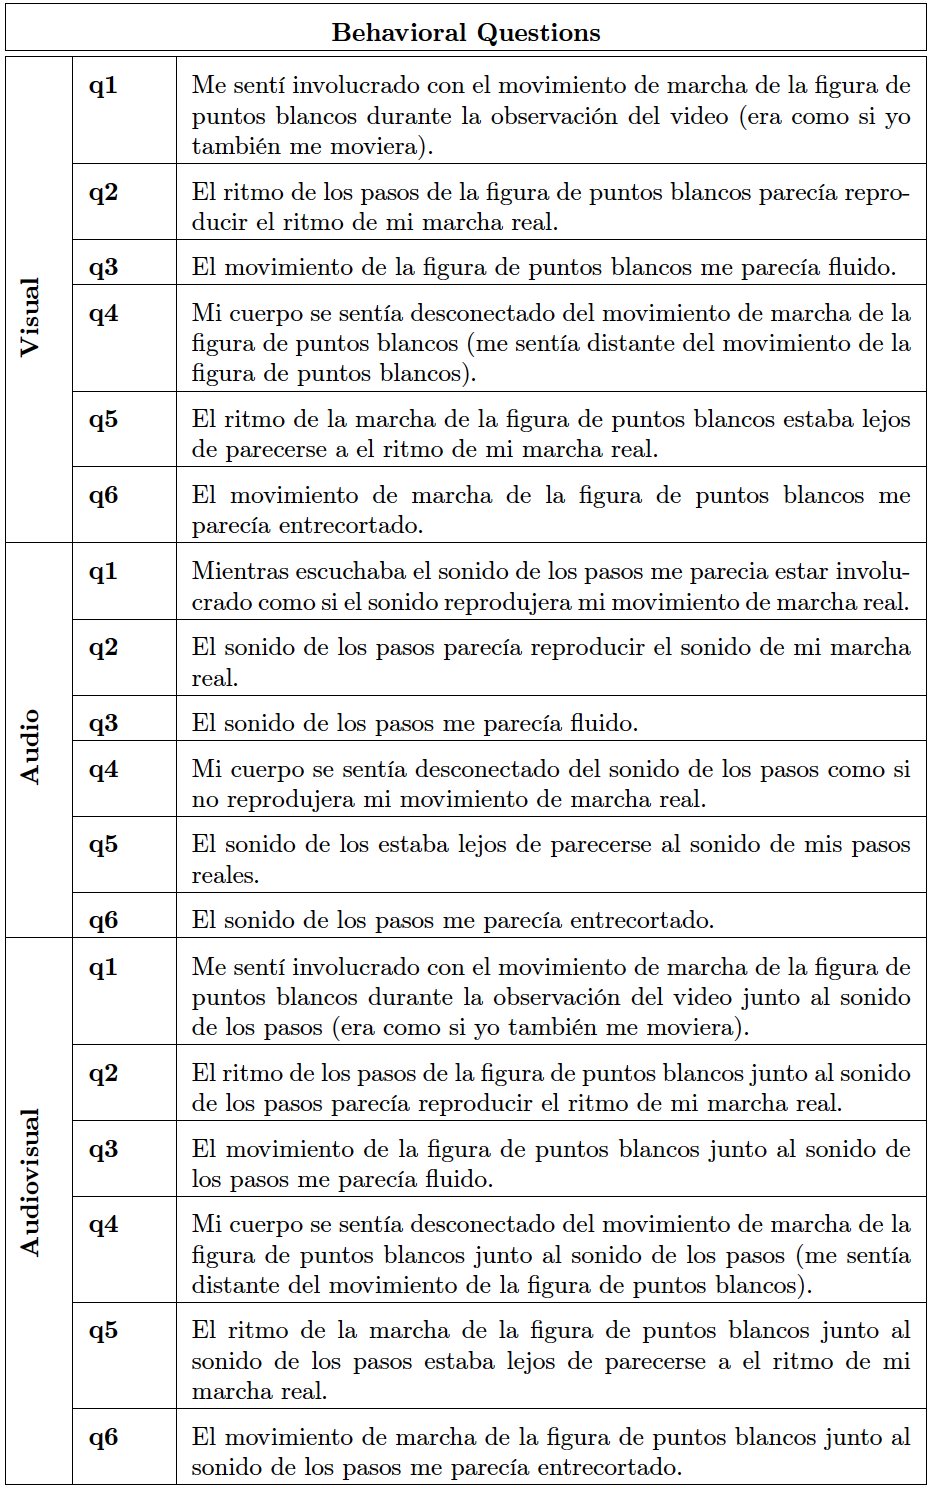
\includegraphics[width=0.70\textwidth]{appendix/questions.png}
    \caption{Behavioral questions translated in English from Spanish}
    \label{fig: Behavioral questions}
\end{figure}
\begin{figure}[ht]
    \centering
    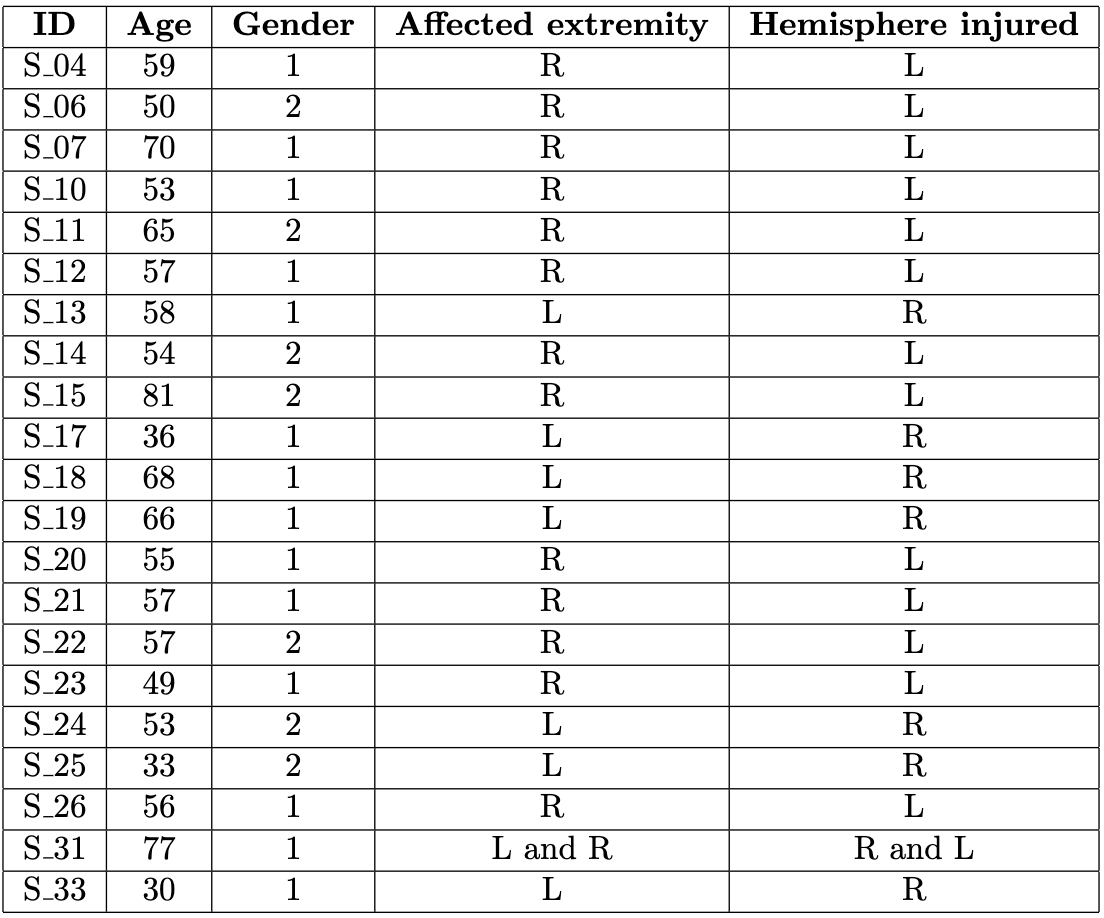
\includegraphics[width=0.70\textwidth]{appendix/database_stroke.png}
    \caption{Database for stroke population (Gender: 1 = man; 2 = woman) }
    \label{fig: Database stroke}
\end{figure}

\clearpage
% \section{Appendix: Active-Q Questionnaire}
% \label{pdf: Active-Q questionnaire}
\includepdf[scale=0.8, pages=1, 
    pagecommand={\section{Appendix: Active-Q questionnaire}\label{pdf: Active-Q questionnaire}}]{appendix/Active-Q test.pdf}
\includepdf[scale=0.8, pages=2-, 
    pagecommand={}]{appendix/Active-Q test.pdf}

\clearpage
\end{appendices}

\printbibliography[heading=bibintoc]

\end{document}